

% \begin{wrapfigure}{r}{0.3\textwidth}
%     \vspace{-3.5em}
%     \centering
%     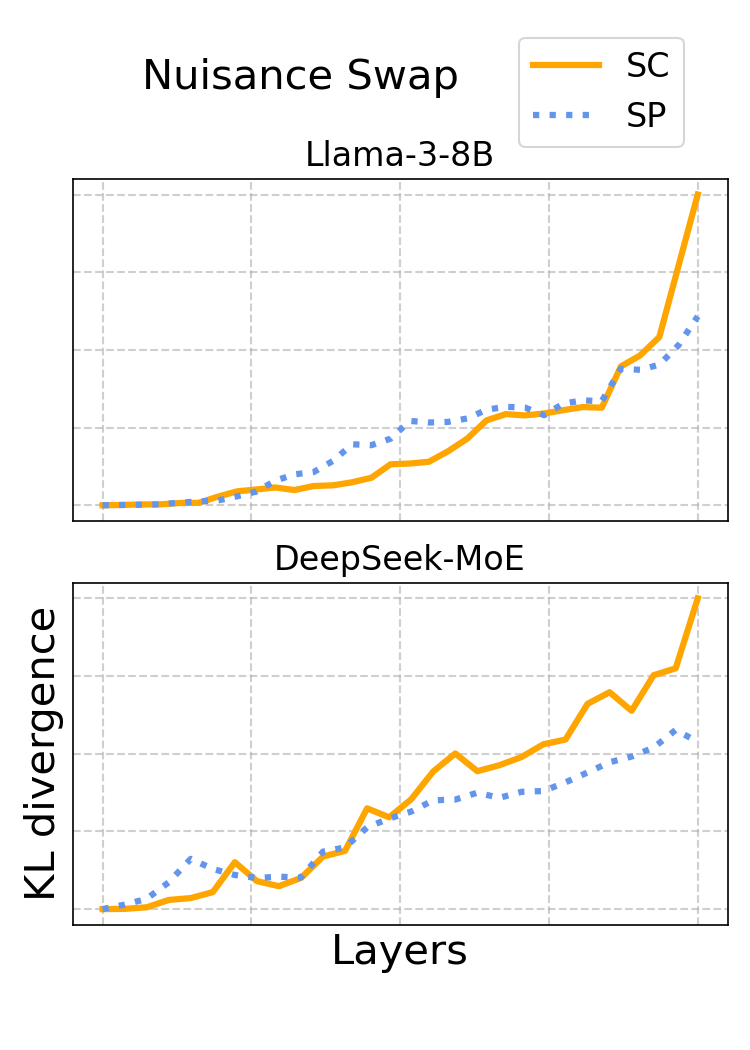
\includegraphics[width=1.0\linewidth]{figures/2_column_nuis_sc_sp_k32_group5.png}
%     \vspace{-3.0em}
%     \caption{\xz{maybe 1-2 plot is fine for here.}Per-layer KL divergence under nuisance component swaps for three representative models ($k=32$, $\alpha=1.0$). Both SC (orange) and SP (blue) curves increase with depth at comparable rates with no consistent separation, indicating that the nuisance subspace affects model outputs but does not exhibit semantic selectivity, and likely contains a mixture of surface-form and residual semantic information.}
%     \label{fig:nuisance_kl}
%     \vspace{-2.25em}
% \end{wrapfigure}

% \begin{wrapfigure}{r}{0.3\textwidth}
%     \vspace{-3.5em}
%     \centering
%     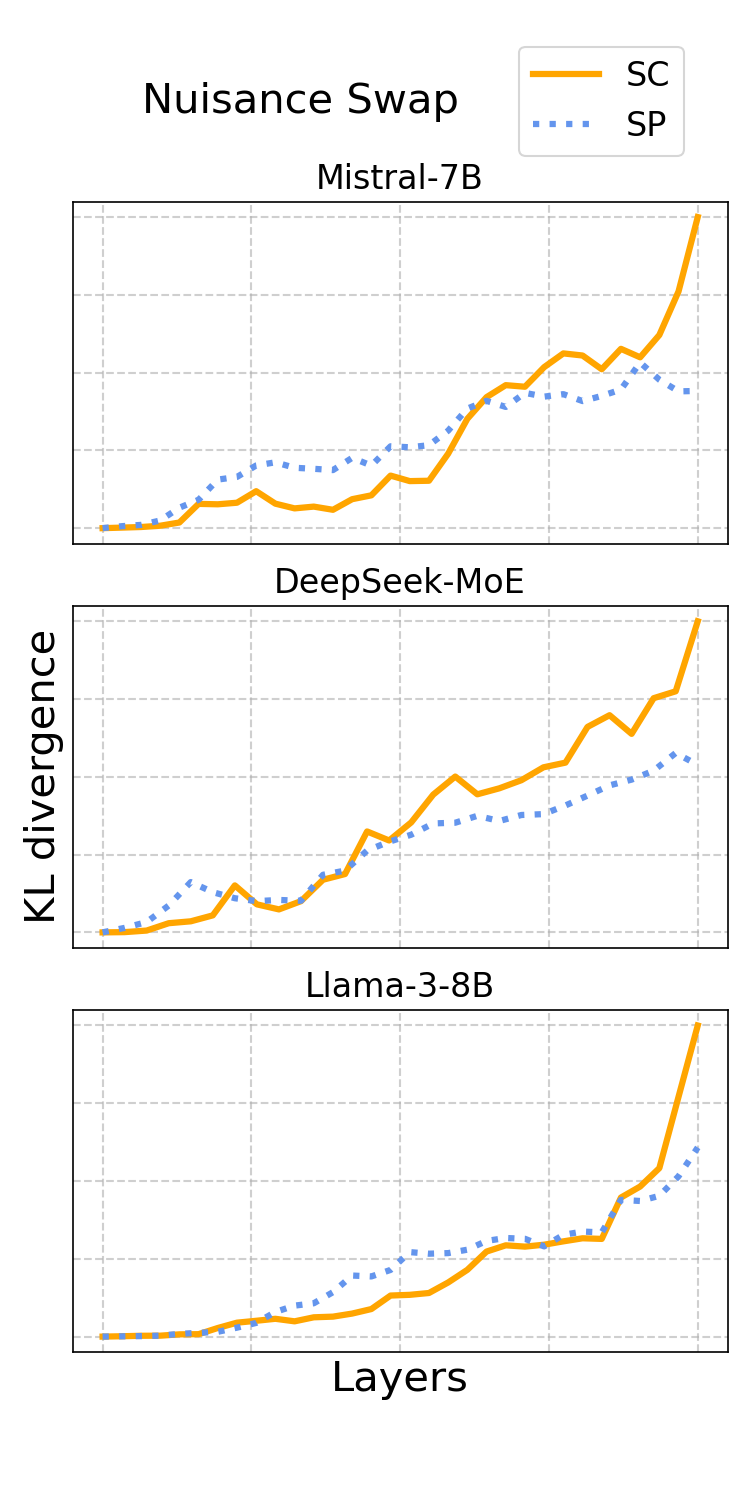
\includegraphics[width=1.0\linewidth]{figures/3_column_nuis_sc_sp_k32_group5.png}
%     \vspace{-3.0em}
%     \caption{\xz{maybe 1-2 plot is fine for here.}Per-layer KL divergence under nuisance component swaps for three representative models ($k=32$, $\alpha=1.0$). Both SC (orange) and SP (blue) curves increase with depth at comparable rates with no consistent separation, indicating that the nuisance subspace affects model outputs but does not exhibit semantic selectivity, and likely contains a mixture of surface-form and residual semantic information.}
%     \label{fig:nuisance_kl}
%     \vspace{-2.25em}
% \end{wrapfigure}

% While the invariant subspace $z_{\mathrm{inv}}$ exhibits strong semantic selectivity, the complementary nuisance subspace $z_{\mathrm{nuis}}$ does not form a perfectly disentangled component. As shown in Fig.~\ref{fig:nuisance_kl}, swapping nuisance components within the same semantic group produces non-negligible output shifts even for semantic-preserving (SP) donors, indicating that the nuisance representation still contains residual semantic information. This suggests that the proposed data-driven decomposition is not perfectly orthogonal in practice, and that the nuisance subspace may capture a mixture of surface-form variation and weak semantic components. Importantly, this asymmetry does not affect the primary findings: invariant-component swaps remain stable under SP perturbations while exhibiting strong separation under semantic-changing conditions (Section~\ref{sec:ab_mainpaper}), confirming that semantic structure is concentrated in the invariant subspace. Achieving a more complete disentanglement of nuisance representations remains an important direction for future work.

\begin{wrapfigure}{r}{0.3\textwidth}
    \vspace{-1.5em}
    \centering
    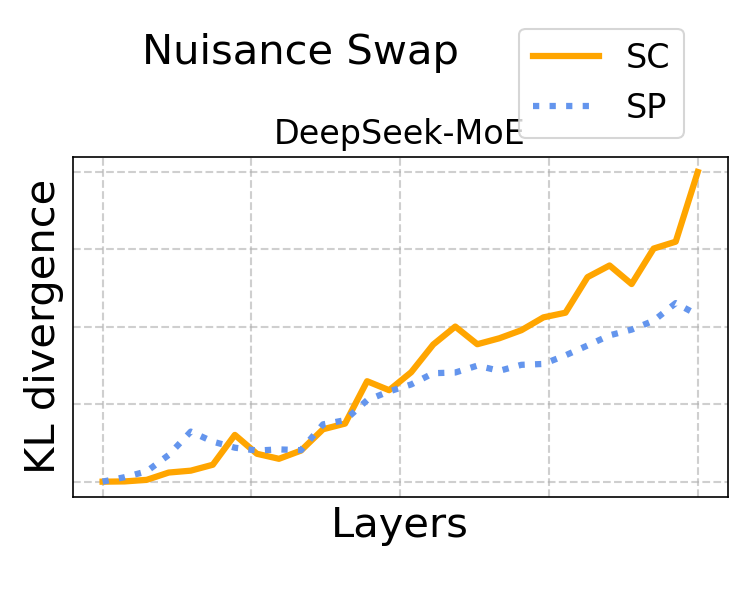
\includegraphics[width=1.0\linewidth]{figures/1_column_nuis_sc_sp_k32_group5.png}
    \vspace{-2.5em}
    \caption{Per-layer KL divergence under nuisance-component swaps for a model. SP and SC curves increase with depth at comparable rates with no consistent separation. The nuisance subspace likely contains a mixture of surface-form and residual semantic information.}
    \label{fig:nuisance_kl}
    \vspace{-1.5em}
\end{wrapfigure}


Our framework provides a local geometric characterization of semantic invariance rather than a universal decomposition of language representations. Although our evaluation spans 1,400 semantic groups, 57,400 sentences, and nine language models, the decomposition remains dependent on the quality and coverage of the SP and SC perturbations. The dataset is synthetically constructed, and generalization to naturally occurring, multilingual, and long-context inputs remains to be systematically evaluated.

While the invariant subspace $z_{\mathrm{inv}}$ exhibits strong semantic selectivity, the complementary nuisance subspace $z_{\mathrm{nuis}}$ does not achieve complete semantic disentanglement. As shown in Fig.~\ref{fig:nuisance_kl}, swapping nuisance components within the same semantic group produces non-negligible output shifts even for semantic-preserving (SP) donors, indicating that the nuisance representation may retain residual semantic information. Although the two subspaces are orthogonal by construction, the nuisance subspace can still capture a mixture of surface-form variation and residual semantic components. Importantly, this asymmetry does not undermine the primary findings: invariant-component swaps remain stable under SP perturbations while exhibiting strong separation under semantic-changing conditions (Section~\ref{sec:ab_mainpaper}), supporting the conclusion that semantic-sensitive information is concentrated in the invariant subspace. Achieving more complete semantic disentanglement remains an important direction for future work.

